The generation of the Graphs and the Monte Carlo Simulation are implemented
in C, all needed random numbers are generated by the GSL \cite{GSL}
implementation of the \emph{Mersenne Twister} \cite{Matsumoto1998} and
the generated data is evaluated via Python scripts.
All source code is available at \url{https://github.com/surt91/IsingFerromagnet}.\\

For evaluation the Monte Carlo simulation is run until the system
is equilibrated after \(t_{eq}\) sweeps. Then the simulation continues
and the magnetisation per site \(m=\frac{1}{N}\sum_i s_i\) and energy
per site \(E=\frac{1}{N}\hat H\) are calculated and saved for every
\(2\tau\) sweeps. Where \(\tau\) denotes the \emph{autocorrelation time}
(see also \ref{ssec:eqtime}).
For every observable \(O\) the expected value \(\avg{O}\) is determined
as the mean of \(10000\) measurements for \(L=16,32\) or \(5000\) for
\(L=64,128\). The expected values \(\avg{O}\) for \(100\) different
random proximity graphs with the same disorder paramter \(\sigma\)
are then averaged to \(\overline{\avg{O}}\). The errors are estimated
by bootstrapping \cite{Bootstrap}.

\subsection{Finite Size Effects}
\label{ssec:finitesize}
    The aim of this thesis is to find the critical temperature \(T_c\)
    of the disordered Ising model in dependence of the disorder parameter
    \(\sigma\). At \(T_c\) the mean absolute magnetisation \(\avg{|m|}\) of
    the system will jump and the susceptibility
    \(\chi = \frac{N}{T}\brac{\avg{m^2}-\avg{m}^2}\)
    will diverge. In fig. \ref{fig:smeared_out}\subref{sfig:smeared_out:meanM}\footnote{See the appendix for a similar figure for the specific heat.}
    it is easy to see that the jump of \(\avg{|m|}\)
    occurs at lower temperatures \(T\) for higher
    disorder parameters \(\sigma\) (here with a Relative Neighborhood graph).
    \begin{figure}[htbp]
        \centering
        \subfigure[Dependence of the phase transition on $\sigma$][]
        {
            \label{sfig:smeared_out:meanM_L}
            \includegraphics[width=0.45\textwidth]{plots/Mean_M_L_128}
        }
        \subfigure[Example for finite size effects][]
        {
            \label{sfig:smeared_out:meanM}
            \includegraphics[width=0.45\textwidth]{plots/meanM}
        }
        \caption[Phase Transition and Finite Size Effects]
        {
            \subref{sfig:smeared_out:meanM_L}: Effects of the disorder
            parameter $\sigma$ on the phase transition
            for an underlying Relative Neighborhood graph with $L=128$.\\
            \subref{sfig:smeared_out:meanM}: Effects of different system
            sizes at \(\sigma = 0\). Dotted lines are guides to the eye.
        }
        \label{fig:smeared_out}
    \end{figure}\\
    But in the shown plots there occurs no real jump, but a continuous
    decline. The jump is only present in infinite systems, hence every
    computer simulation will show some \emph{finte size effects}.
    These finite size effects cause a "smearing out" of the phase
    trasition. This is stronger for smaller system sizes, as is visible
    in fig. \ref{fig:smeared_out}\subref{sfig:smeared_out:meanM}. Clearly
    the \(L=16\) curve is much less steep than the \(L=128\) curve.\\
    Despite of this one can obtain \(T_c\) by finite size scaling
    methods \cite[S. ??]{NewmanBarkema1999} which also yield the critical
    exponents.
    Studies on random lattices with variing coupling constants \(J\)
    \cite{Lima2000} and without \cite{Janke1994} suggest, that the
    critical exponents should not be influenced by the disorder paramter
    \(\sigma\). So they will be used for consistency cross checking and
    comparision with the known exact values \cite[S. 59]{Pelissetto2002}.\\
    % Ausfuehrlichere Herleitung der Skalentheorie, Skalenanalyse
    For a more in depth look at finite size scaling, \cite{Norrenbrock2011}
    offers a explanation.
    It is known, that for large \(L\) near the critical temperature the
    equations \eqref{eq:fsscaling:m}, \eqref{eq:fsscaling:chi} and
    \eqref{eq:fsscaling:g} apply.
    \begin{align}
        \label{eq:fsscaling:m}
        \avg{m_L} &= L^\frac{\beta}{\nu} \tilde{M}\brac{L^\frac{1}{\nu}\brac{T-T_c}}\\
        \label{eq:fsscaling:chi}
        \chi_L    &= L^\frac{\gamma}{\nu} \tilde{C}\brac{L^\frac{1}{\nu}\brac{T-T_c}}\\
        \label{eq:fsscaling:g}
        g          &= \frac{3}{2}\brac{1-\frac{\avg{m^4}}{3\avg{m^2}^2}} \propto \tilde{G}\brac{L^\frac{1}{\nu}\brac{T-T_c}}
    \end{align}
    Where \(g\) from eq. \eqref{eq:fsscaling:g} is a normalized
    Binder cumulant \cite{Binder1981} and \(\tilde{M}, \tilde{C}\) and \(\tilde{G}\)
    are unkown scaling functions. To find the exponents
    \(\beta, \gamma, \nu\) and the critical temperature \(T_c\), one
    varies them until the measured values of the observables collapse on
    one curve. Like the obersables from fig. \ref{fig:gettingCrit}\subref{sfig:gettingCrit:binder_fit_s_0}
    collapse in fig. \ref{fig:gettingCrit}\subref{sfig:gettingCrit:collapse_s_0}.
    Note that \(L=16\) is not used for the collapse, because it is a
    rather small value such that eq. \eqref{eq:fsscaling:m}-\eqref{eq:fsscaling:g}
    do not apply very good.\\
    To accomplish the collapse in an semi-automatic and reproduceable
    way with an error estimate, the programm
    \texttt{autoscale.py} \cite{autoscale2009} is used.
    \begin{figure}[htbp]
        \centering
        \subfigure[Example of a Binder cumulant to determine the critical temperature][]{
            \label{sfig:gettingCrit:binder_fit_s_0}
            \includegraphics[width=0.47\textwidth]{plots/binder_fit_s_0}
        }
        \subfigure[Example of a datacollapse to determine critical exponents][]{
            \label{sfig:gettingCrit:collapse_s_0}
            \includegraphics[width=0.47\textwidth]{plots/collapse_s_0}
        }
        \caption[Examples of determining critical temperature and exponents]
        {
            The Binder cumulant \(g\) of an square lattice Ising model
            (\(\sigma=0\))\\
            \subref{sfig:gettingCrit:binder_fit_s_0} interpolated
                with cubic splines (the errorbars are too small to see)\\
            \subref{sfig:gettingCrit:collapse_s_0} collapsed by finite
                size scaling
        }
        \label{fig:gettingCrit}
    \end{figure}\\
    Though if one is just interested in the critical Temperature, an
    easier approach is to find the intersections of the Binder cumulants
    \(g\) of different system sizes \(L\) because they are intersecting
    at \(T_c\) \cite{Binder1981}.
    Because  the magnetisation \(m\) is only measured for discrete values
    of \(T\), \(g\) is also only known for these discrete values and has
    to be interpolated to find a intersection. Therefore a cubic spline
    interpolation\footnote{created using the \texttt{scipy.interpolate} tools \cite{scipy2001}}
    is calculated for the measured points.
    Cubic spline interpolation is a piecewise fitting of polynoms of
    degree three which are joined under the condition to be at least two
    timescontinuously differentiable.
    As an example take fig. \ref{fig:gettingCrit}\subref{sfig:gettingCrit:binder_fit_s_0}.
    Here such interpolations are plotted for \(\sigma=0\) and are
    intersecting at \(\approx 2.27\).
    To determine \(T_c\), the intersections\footnote{found using the \texttt{scipy.optimize} tools \cite{scipy2001}}
    are averaged and the standard error is calculated. In this case one
    gets \(T_c = 2.2689(2)\), which is in good agreement with the
    exact solution from eq. \eqref{eq:exactTc} \cite{Onsager1944}.
    \begin{equation}
        T_c = 2J/\ln(1+\sqrt 2) = 2.2691...
        \label{eq:exactTc}
    \end{equation}

\subsection{Critical Temperature}
\label{ssec:binderIntersections}
    The evaluation of the Binder cumulant's intersections, yields the
    critical temperatures \(T_c\), which are plotted in
    fig. \ref{fig:Tc}\subref{sfig:Tc:RNG}\subref{sfig:Tc:GG}.
    Further in fig. \ref{fig:Tc}\subref{sfig:sumJ:RNG}\subref{sfig:sumJ:GG}
    the mean sum of the coupling constants to all neighbors \(\avg{\sum_{\avg{i,j}} J_{ij}}\)
    is plotted which is evidently correlated with \(T_c\).
    That is plausible, because \(T_c\) is dependend on the coupling
    constant \(J\) (compare \eqref{eq:exactTc}).\\
    It seems reasonable to normalize the values of \(T_{c}\) by
    \(\avg{\sum_{\avg{i,j}} J_{ij}}\) which yields the diagramms fig.
    \ref{fig:Tc}\subref{sfig:Tc_norm:RNG}\subref{sfig:Tc_norm:GG}.
    \begin{figure}[htbp]
        \centering
        \subfigure[][]
        {
            \label{sfig:Tc:RNG}
            \includegraphics[width=0.45\textwidth]{plots/RNG_Tc}
        }
        \subfigure[][]
        {
            \label{sfig:Tc:GG}
            \includegraphics[width=0.45\textwidth]{plots/GG_Tc}
        }

        \subfigure[][]
        {
            \label{sfig:sumJ:RNG}
            \includegraphics[width=0.45\textwidth]{plots/RNG_sumJ}
        }
        \subfigure[][]
        {
            \label{sfig:sumJ:GG}
            \includegraphics[width=0.45\textwidth]{plots/GG_sumJ}
        }

        \subfigure[][]
        {
            \label{sfig:Tc_norm:RNG}
            \includegraphics[width=0.45\textwidth]{plots/RNG_Tc_norm}
        }
        \subfigure[][]
        {
            \label{sfig:Tc_norm:GG}
            \includegraphics[width=0.45\textwidth]{plots/GG_Tc_norm}
        }
        \caption[Critical Temperature over different disorder parameters]
        {
            Top: Critical temperatures over different
            disorder parameters for
            \subref{sfig:Tc:RNG} the Relative Neighborhood Graph and
            \subref{sfig:Tc:GG} the Gabriel Graph.\\
            Middle: Mean sum of the coupling constants to all
            neighbors over different disorder parameters for
            \subref{sfig:sumJ:RNG} the Relative Neighborhood Graph and
            \subref{sfig:sumJ:GG} the Gabriel Graph.\\
            Bottom: Normalized critical temperatures over different
            disorder parameters for
            \subref{sfig:Tc_norm:RNG} the Relative Neighborhood Graph and
            \subref{sfig:Tc_norm:GG} the Gabriel Graph.
        }
        \label{fig:Tc}
    \end{figure}\\
    % I don't know what all that means...
    The Gabriel graph, which is shown on the right side of fig. \ref{fig:Tc},
    jumps from \(\sigma = 0\) to \(\sigma > 0\). This is easily explained
    by the definition of the Gabriel graph and it's aftereffects for
    the transition from \(\sigma = 0\). Visible in fig. \ref{fig:GG_sigma}
    a small change of sigma causes many new egdes to arise\footnote{See also \url{http://www.youtube.com/watch?v=PcVZ2pG11GI} for an animation.}.
    To fully understand this, take four nodes forming a square. The edge
    across does not exist, because the other two nodes are on the edge
    of the lune. Moving one node slightly into the square, causes the lune
    to get smaller, hence no other nodes are inside or on the edge of
    the lune anymore and the edge appears.
    \begin{figure}[htbp]
        \centering
        \subfigure[][]
        {
            \label{sfig:GG_sigma:zero}
            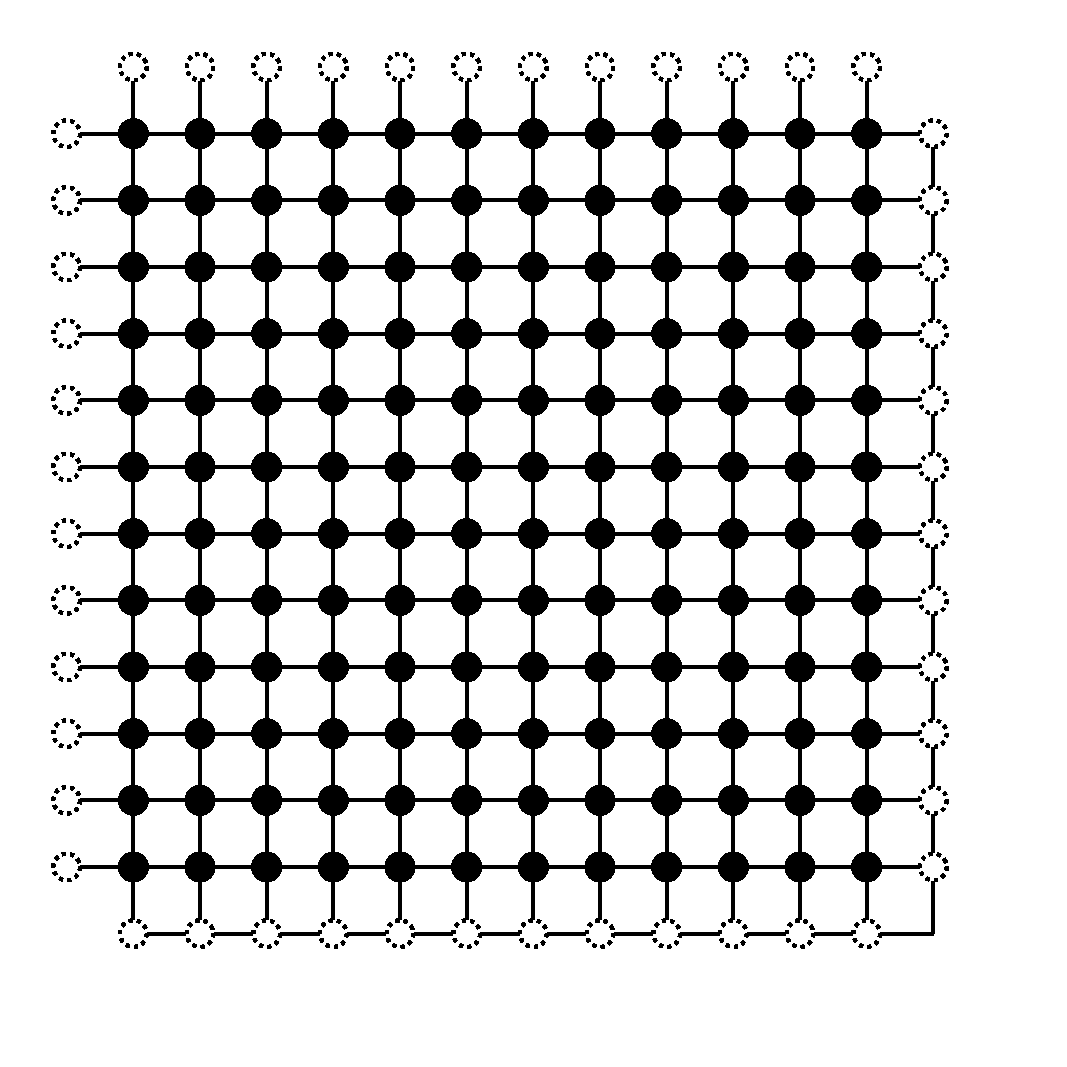
\includegraphics[width=0.40\textwidth]{images/GG/sigma_e0}
        }
        \subfigure[][]
        {
            \label{sfig:GG_sigma:notzero}
            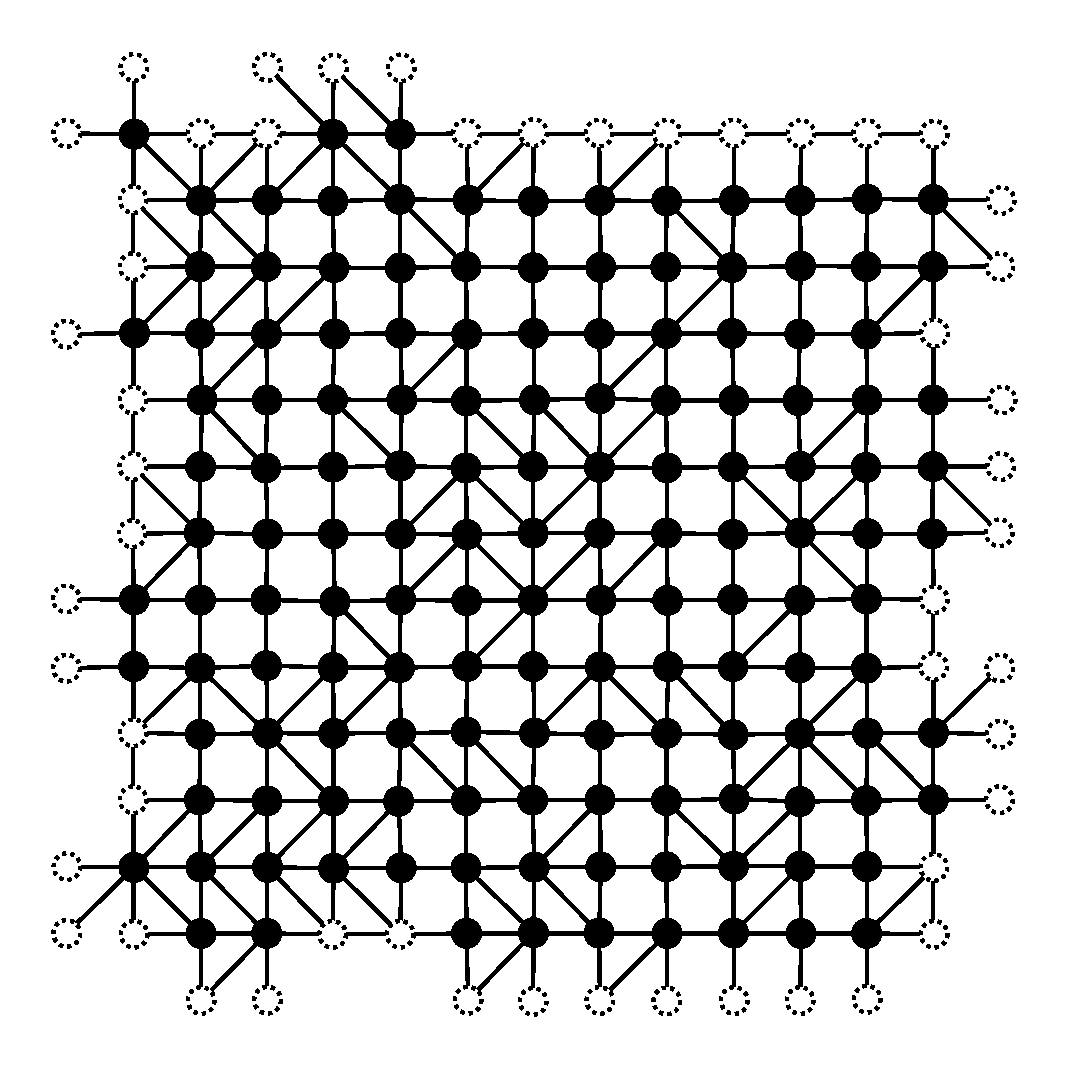
\includegraphics[width=0.40\textwidth]{images/GG/sigma_g0}
        }
        \caption[]
        {
            Gabriel graph with periodic boundary conditions for
                \subref{sfig:GG_sigma:zero} \(\sigma = 0\)
                \subref{sfig:GG_sigma:notzero} \(\sigma = 0.01\)
        }
        \label{fig:GG_sigma}
    \end{figure}\\
    Moreover fig. \ref{fig:Tc}\subref{sfig:Tc_norm:RNG}\subref{sfig:Tc_norm:GG}
    shows monotonically decreasing \(T_c\) with increasing disorder
    parameter \(\sigma\). The forms of both curves are similar, but the
    one for the Relative Neighborhood graph \ref{fig:Tc}\subref{sfig:Tc_norm:RNG}
    is generally lower and spans over a bigger temperature range than
    the curve of the Gabriel graph \ref{fig:Tc}\subref{sfig:Tc_norm:GG}.
    % Warum??? Die eigenschaften des Graphen sollten mit der Normalisierung erledigt sein.
    % RNG: laengere Kanten -> weniger lokale effekte?
    For big \(\sigma\) the curve approaches the limit of randomly
    distributed nodes, hence \(T_c\) is independet of \(\sigma\) for
    \(\sigma >> 1\).\\
    Also both graph types have a plateau at \(0 < \sigma < 0.1\). So
    small disorder has little influence on the normalized critical temperature.
    But once the degree of the graph and hence the mean sum of the coupling
    constants decreases, the normalized critical temperature decreases, too.
    % The author is not sure what it means.
    % mit theo ergebnissen von Honeycomb \cite{Wannier1945} vergleichen (fur deg = 3)
    % cosh(2L_c)=2 mit L_c = J/2kT_c -> T_c \approx 1.52

\subsection{Critical Exponents}
    For \(\sigma \in \{0,0.1,0.2,0.3,0.5,1.0\}\) a finite size scaling analysis was
    performed to determine the critical exponents \(\beta, \gamma, \nu\)
    using \texttt{autoscale.py} \cite{autoscale2009}. The values for
    \(\sigma = 0\) are analytically known \cite{Pelissetto2002}. The
    values for all other \(\sigma\) should be the same as for \(\sigma = 0\)
    like mentioned before in section \ref{ssec:finitesize}.
    The values for \(\sigma\) are chosen to represent every interesting
    region from fig. \ref{fig:Tc}\subref{sfig:Tc_norm:RNG}\subref{sfig:Tc_norm:GG}:
    the plateau at small \(\sigma\), the steep decline and the plateau at
    big \(\sigma\).\\
    Like in tab. \ref{tab:critExp} to see, most values
    are matching the expectations. Most \(\beta\) seem to be a bit too
    big, but they are close enough to the expectations to be explained
    by the fact that small systems (\(L=32,64\)) were used for the
    analysis.
    Anyway, two critical exponents are sufficient to determine the universality
    class. Therefore this disordered Ising modell is in the same universality
    class as the standard Ising ferromagnet \cite[p. 145]{Katzgraber2011}.
    \begin{table}[htbp]
        \center
        \begin{tabular}{l l l l l}
            \toprule
             & \multicolumn{1}{c}{\(\sigma\)} & \multicolumn{1}{c}{\(\nu\)} & \multicolumn{1}{c}{\(\gamma\)} & \multicolumn{1}{c}{\(\beta\)}\\
            \midrule
            exact (\cite[p. 59]{Pelissetto2002}) & \multicolumn{1}{c}{\(0\)} & \multicolumn{1}{c}{\(1\)} & \multicolumn{1}{c}{\(-\frac{7}{4}\)} & \multicolumn{1}{c}{\(\frac{1}{8}\)}\\
            \midrule
            Gabriel      & 0.0 & 1.008(4) & -1.735(2) & 0.1262(4)\\
                         & 0.1 & 1.02(1)  & -1.744(5) & 0.133(6) \\
                         & 0.3 & 1.000(5) & -1.724(16)& 0.129(12)\\
                         & 0.5 & 1.009(8) & -1.750(12)& 0.125(13)\\
                         & 1.0 & 1.015(22)& -1.743(17)& 0.123(16)\\
            \midrule
            Relative N.  & 0.0 & 1.007(2) & -1.739(2) & 0.130(1) \\
                         & 0.1 & 0.99(1)  & -1.746(5) & 0.133(4) \\
                         & 0.2 & 1.022(17)& -1.756(14)& 0.123(10)\\
                         & 0.5 & 1.002(17)& -1.750(16)& 0.143(13)\\
                         & 1.0 & 1.011(20)& -1.758(16)& 0.138(13)\\
            \bottomrule
        \end{tabular}
        \caption{Critical exponents for different \(\sigma\)}
        \label{tab:critExp}
    \end{table}

\subsection{Critical Value of the Binder Cumulant}
    The value of the Binder cumulant at the critical point \(g_c\) is
    depends strongly on boundary conditions but only weakly on the lattice
    structure \cite{BinderValue}. For periodic boundary conditions on a
    square lattice it is \(g_c \approx 0.916\) according to \cite{BinderValue}
        \footnote{Note that \cite{BinderValue} uses an other definition of
            the Binder cumulant, and has to be normalized by \(\frac{2}{3}\)
            to match it's definition in this thesis.}.
    Because the analysis of section \ref{ssec:binderIntersections}
    yields \(g_c\) anyway, it is easy to check the consistency and
    behaivior of \(g_c\) in the disordered Ising modell.\\
    \begin{figure}[htbp]
        \centering
        \subfigure[for a Relative Neighborhood graph][]
        {
            \label{sfig:TcG:RNG}
            \includegraphics[width=0.45\textwidth]{plots/RNG_TcG}
        }
        \subfigure[for a Gabriel graph][]
        {
            \label{sfig:TcG:GG}
            \includegraphics[width=0.45\textwidth]{plots/GG_TcG}
        }
        \caption[Values of the Binder cumulant at the critical point $g_c$]
        {
            Values of the Binder cumulant at the critical point \(g_c\)
            for\\
            \subref{sfig:TcG:RNG} a Relative Neighborhood graph and\\
            \subref{sfig:TcG:GG} a Gabriel graph for different \(\sigma\).
            The dotted line is the reference value for square lattices
            with periodic boundary conditions \cite{BinderValue}, which
            corresponds to \(\sigma = 0\).
        }
        \label{fig:TcG}
    \end{figure}\\
    Considering both plots in fig. \ref{fig:TcG}, \(g_c\) is for low
    \(\sigma\) obviously always bigger than the known value. Though the
    deviation is less than \(1\%\). Perhaps this is some inherent flaw
    of the cubic spline interpolation used to aquire these \(g_c\) values.
    For bigger \(\sigma\) the uncertainty gets greater, but the values
    do only differ by a few percent, hence even the big disorder and
    definition of nearest neighbors via a proximity graph does not change
    \(g_c\) much. This is the expected behaivior.


%~ Darstellung von Suszeptibilität \(\chi\), spezifischer Wärme \(c\), mittlerer Magnetisierung \(<m>\) über Unordnungsparamter \(\sigma\)\\
